\documentclass[9pt]{beamer}

\usetheme{metropolis}
\usepackage{appendixnumberbeamer}

\usepackage{booktabs}
\usepackage[scale=2]{ccicons}


\usepackage{tikz}
\usetikzlibrary{shapes,arrows}
\usepackage{amsmath, bm}
\usepackage{physics}
\usepackage{mathtools}

\usepackage{pgfplots}
\usepgfplotslibrary{dateplot}

\usepackage{xspace}
\usepackage{soul}
\newcommand{\themename}{\textbf{\textsc{metropolis}}\xspace}

\DeclareMathOperator{\msbar}{\overline{MS}}

\title{Can $\msbar$ PDF be negative?}
%\subtitle{make PDFs positive and everyone happy}
\date{February, 2020}
\author{Alessandro Candido
}
%\institute{N3PDF}
\titlegraphic{
%        \raisebox{5pt}[0pt][0pt]{
\includegraphics[height=0.8cm]{../_logos/nnpdf_logo.pdf}}\hspace*{10pt}
        \hfill
        \raisebox{5pt}[0pt][0pt]{
\includegraphics[height=0.8cm]{../_logos/n3pdf_logo.pdf}}\hspace*{10pt}
        
\includegraphics[height=1.1cm]{../_logos/erc_logo.png}

        \vfill\vspace*{170pt}
        
\includegraphics[height=1cm]{../_logos/unimi_logo.png}\hfill
        
\includegraphics[height=1cm]{../_logos/infn_logo.png}\\
        \vspace*{5pt}
        {\fontsize{3pt}{3.5pt}\selectfont
             \begin{center}
                 This project has received funding from the European Union's Horizon 2020 research and innovation programme under grant agreement No 740006\quad 
\includegraphics[height=5pt]{../_logos/eu-flag.jpg}
         \end{center}}
}

\begin{document}

\maketitle

\begin{frame}{Table of contents}
  \setbeamertemplate{section in toc}[sections numbered]
    \tableofcontents%[hideallsubsections]
\end{frame}

\section{Parton model}
\begin{frame}{Introduction}
    \begin{columns}
        \begin{column}{0.7\textwidth}
            The \textit{parton model} consist in a model of the proton
            structure as a bunch of free components, collectively called
            \textit{partons}:

            \begin{itemize}
                \item in principle any elementary particle
                \item in practice mostly \textbf{quarks} and \textbf{gluons}
            \end{itemize}

            This assumption of course relies on the asymptotic freedom of
            strong interaction\footnotemark.
        \end{column}
        \begin{column}{0.3\textwidth}
            \begin{figure}
                \centering
                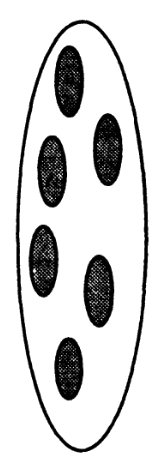
\includegraphics[height=150pt]{pictures/partons}
            \end{figure}
        \end{column}
    \end{columns}
    \footnotetext{e.g. it would be completely unphysical for an atom.}

\end{frame}


\begin{frame}{LO PDF definition}
    \begin{columns}
        \begin{column}{0.55\textwidth}
            Since they are free the main property of each parton is the
            fraction of the total momentum it carries.\newline

            The probability distribution of finding a parton $p$ with momentum
            fraction $x$ it's encoded in its \textit{Parton Density Function}\footnotemark,
            $f_p(x)$.
        \end{column}
        \begin{column}{0.45\textwidth}
            Plot LO PDFs 
            %\begin{figure}
                %\centering
                %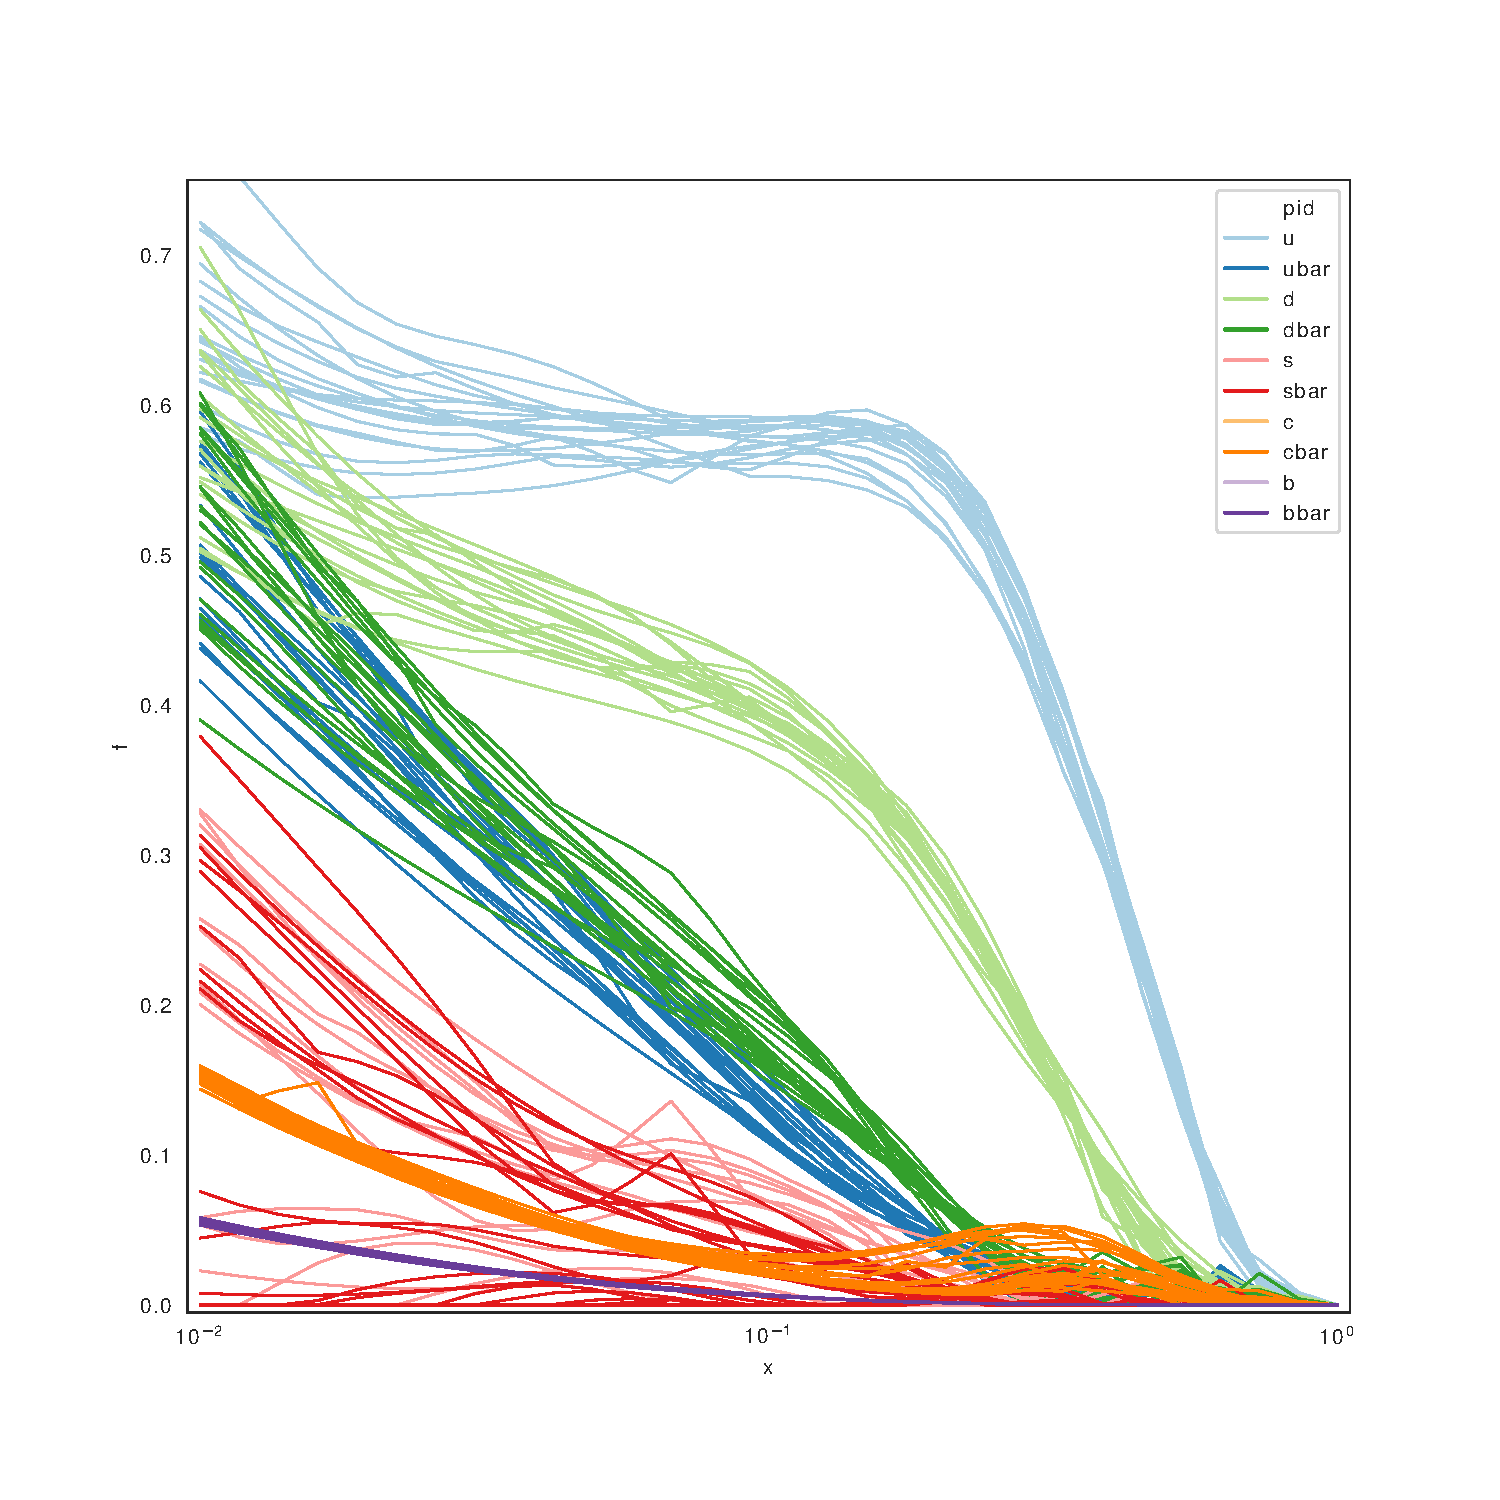
\includegraphics[height=150pt]{pictures/lo_pdfs}
            %\end{figure}
        \end{column}
    \end{columns}
    \footnotetext{In general PDFs also depend on the energy scale $Q^2$,
    but at LO they scale (see \textit{Björken scaling}).}
\end{frame}

\section{PDF @ NLO: factorization scheme}
\begin{frame}{Introduction}
    A step further: NLO -> collinear divergences -> coefficient functions ambiguity (collinear subtraction) -> factorization scheme (as PDF definition)

    Catani-Seymour formula for factorization @ NLo
\end{frame}

\section{An intrinsic positive scheme}
\begin{frame}{Introduction}
    DIS scheme and similar.

    Defined on physical observables.
\end{frame}

\section{Coefficient functions NLO behaviour}
\begin{frame}{Universality of collinear structure}
    We can play this game because we know in advance that the relevant structure (the one related to the collinear subtraction) is universal.
\end{frame}

\begin{frame}{Scheme change matrix}
    How we switch scheme and $K$ properties
\end{frame}

\begin{frame}{A bunch of nontrivial positivity schemes}
    POS, MPOS, DPOS
\end{frame}

\section{Is $\msbar$ negative?}
\begin{frame}{N-space positivity $\neq$ x-space positivity}
    The easy way in \textit{N-space} and Why we need an argument in \textit{x-space}
\end{frame}

\begin{frame}{Introduction}
    Argument from MPOS -> MSbar
\end{frame}


\begin{frame}[standout]
    Thanks for your attention
\end{frame}


\end{document}
